% Presentación para la defensa del proyecto de fin de carrera: "Diseño, desarrollo y explotación de una solución basada en SBC (Raspberry Pi) para la sustitución del instrumental de los laboratorios de física de la Facultad de Ciencias".
% Autor: Diego Muñoz Callejo
% Facultad de Ciencias, Universidad de Cantabria.
% Septiembre de 2014

%Presentación del proyecto: Motivación, objetivos.
%Desarrollo: Proyecto paralelo, qué partes se han desarrollado, el método de trabajo, dificultades encontradas.
%El programa final y la librería piDA, trabajos futuros (implementación en los laboratorios, ¿explotación comercial?)
%Resultados y tal
%Demostración.

\documentclass{beamer}
\usetheme[backgroundimagefile=img/Raspi_Colour_R,useblacktitletext,opacity=0]{diepen}
\setbeamercovered{transparent} % <-- the next layers are grayed out

\usepackage[utf8]{inputenc}
\usepackage[spanish]{babel}
\usepackage[official]{eurosym}
\usepackage{fixltx2e}	%subscript
\setbeamertemplate{footline}[frame number]
\graphicspath{ {img/} }

\newenvironment{slide}	%Frames con la sección como título y subsección como subtítulo.
{\begin{frame}[environment=slide]
\frametitle{\insertsectionnumber.\insertsection}
\framesubtitle{\setlength{\parindent}{2ex} \insertsectionnumber.\insertsubsectionnumber.\insertsubsection}}
{\end{frame}}


\setbeamertemplate{section in toc}{\inserttocsectionnumber.~\inserttocsection}
\setbeamertemplate{subsection in toc}{\setlength{\parindent}{2ex} \inserttocsectionnumber.\inserttocsubsectionnumber.\inserttocsubsection\\}

\DeclareUnicodeCharacter{20AC}{\euro{}} % para escribir € sin tanta movida

\AtBeginSection[]
{
  \begin{frame}
    \frametitle{Índice de contenidos.}
    \tableofcontents[currentsection]
  \end{frame}
}


\begin{document}
\title[piDA Graphic Interface]{piDA Graphic Interface\\[2ex]}
\subtitle{Diseño, desarrollo y explotación de una solución basada en SBC (Raspberry Pi) para la sustitución del instrumental de los laboratorios de física de la Facultad de Ciencias.}   
\author[Diego Muñoz Callejo]{\textbf{Diego Muñoz Callejo}\\[1ex] \footnotesize Co-Directores:\\ Rafael Menéndez de Llano Rozas \\ Esteban Stafford Fernández}
%\author{\begin{tabular}{r@{ }l} 
%Autor:	& Diego Muñoz Callejo \\[1ex] 
%	Co-Directores: & Rafael Menéndez de Llano Rozas
%		& Esteban Stafford Fernández
%\end{tabular}} 
\institute{Facultad de Ciencias, Universidad de Cantabria}
\date{\today} 
\logo{\hfill
\includegraphics[height=1cm]{logo-uc.png}}

\frame{\titlepage}

\frame{\frametitle{Índice de contenidos.}\tableofcontents} 

\section{Introducción.}

\subsection{Problemática.}
\begin{slide}
	\begin{itemize}
		\item Parte del actual instrumental de los laboratorios de Física tiene problemas de mantenimiento.
		\item El coste del reemplazo de dicho instrumental es relativamente alto.   
	\end{itemize}
\end{slide}


\subsection{Objetivos.}
\begin{slide}
	\begin{itemize}
		\item Diseñar y desarrollar una alternativa al equipo existente en los laboratorios con un coste inferior.
		\item La solución debe cubrir las áreas estudiadas por los alumnos en las prácticas.
		\item El coste ha de ser lo más reducido posible.
	\end{itemize}
\end{slide}

\subsection{Motivación.}
\begin{slide}
	\begin{itemize}
		\item Proveer una alternativa realmente económica para la renovación o sustitución del actual material existente en los laboratorios de la Facultad, cuyo coste es muy alto como para poder ser asumido.
	
		\item Los SBCs (Single Board Computers) como la Raspberry Pi ofrecen a un coste reducido un ordenador completamente funcional de modestas prestaciones.
	\end{itemize}
	\begin{center}
		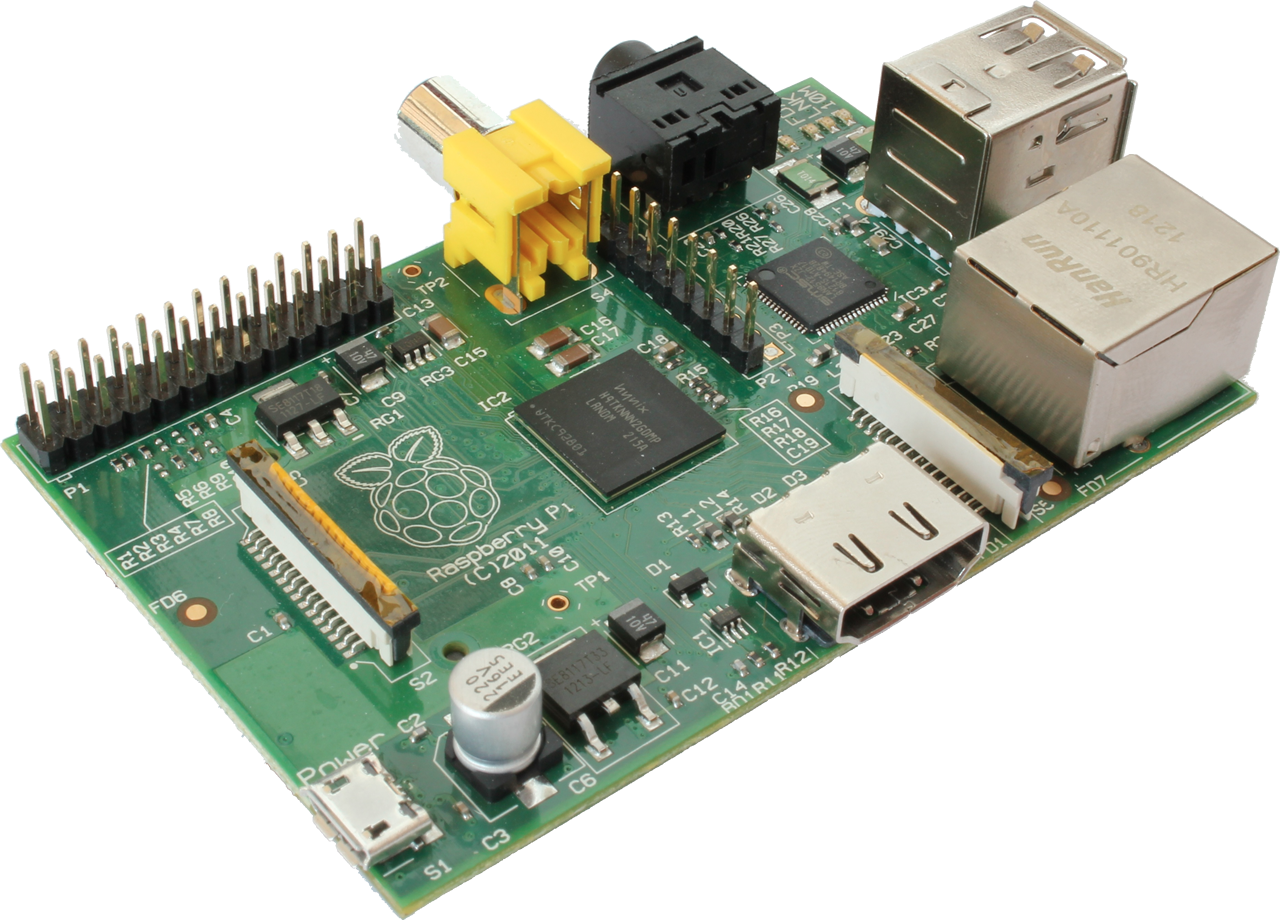
\includegraphics[scale=0.1]{Rpi-B-transp.png}
	\end{center}	
	
\end{slide}

\subsection{Resumen.}
\begin{slide}
	\begin{itemize}
		\item piDA Graphic Interface es un programa creado para realizar medidas a través de sensores desde una Raspberry Pi.
		\item El programa se apoya en la librería piDA.%, de la que toma parte del nombre , creada en un proyecto paralelo a éste.
		\item Se han creado varios prototipos de hardware para la interconexión de sensores.
		\item El resultado final es un sistema de adquisición de datos capaz de sustituir material de laboratorio por valor de más de 1000€.
	\end{itemize}
\end{slide}

\section{Desarrollo.}
\subsection{Proyecto paralelo.}
\begin{slide}
	\begin{itemize}
		\item La solución final ha constado de dos partes diferenciadas realizadas por dos proyectos paralelos.
		\item Se ha diseñado un nexo de conexión para que la progresión de ambos proyectos sea independiente.
	\end{itemize}
	\begin{center}
		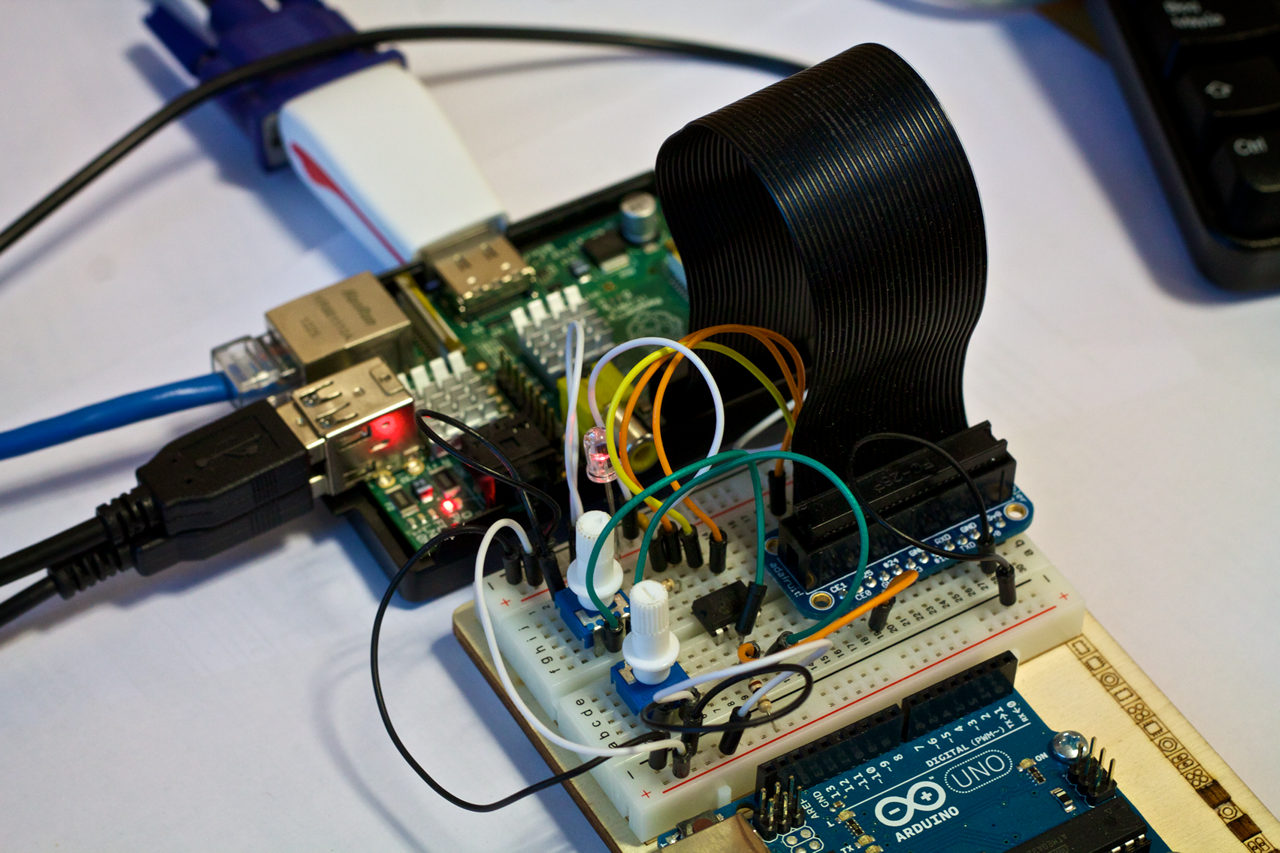
\includegraphics[scale=0.114]{proto1.png}
	\hfill	
		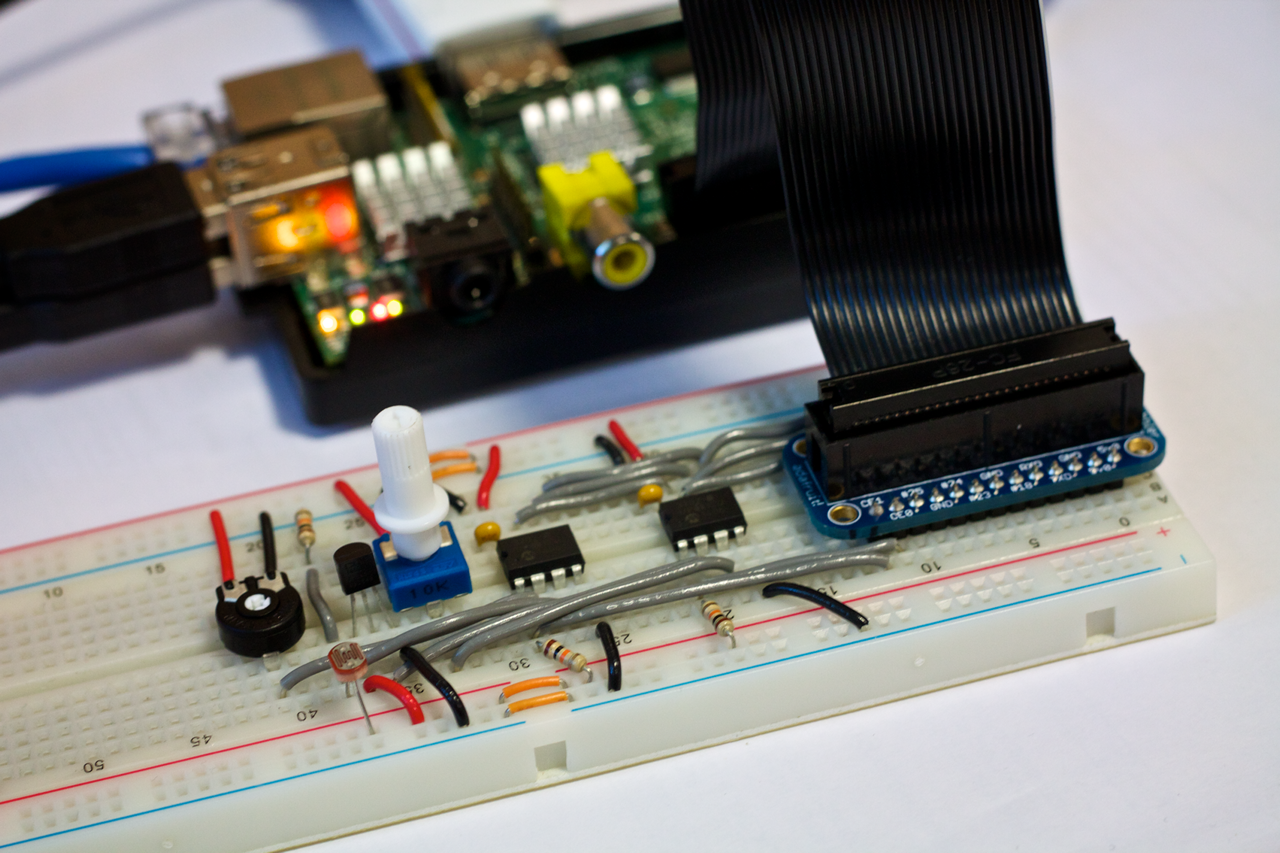
\includegraphics[scale=0.114]{proto2.png}
	\end{center}
\end{slide}

\subsection{Metodología.}
\begin{slide}
	\begin{itemize}
		\item Antes de comenzar el desarrollo: Ingeniería de software. \pause
	%	\begin{itemize}
	%		\item Reuniones con los clientes.
	%		\item Estudio del contexto.
	%		\item Análisis de las soluciones actuales.
	%		\item Propuesta de una nueva solución.
	%	\end{itemize}
		\item Durante el desarrollo: Aprendizaje y familiarización con el entorno. \pause
	%	\begin{itemize}
	%		\item Hitos diarios.
	%		\item Test de la aplicación al final de cada hito.
	%		\item Repositorio de software Github siempre con una versión funcional.
	%	\end{itemize}
		\item Al final del desarrollo: Evaluación de la solución.	
	%	\begin{itemize}
	%		\item Evaluación y análisis de los límites funcionales del programa.
	%		\item Establecimiento de líneas futuras y posibles mejoras.
	%	\end{itemize}
	\end{itemize}
\end{slide}

\subsection{Diagrama de clases.}
\begin{slide}
	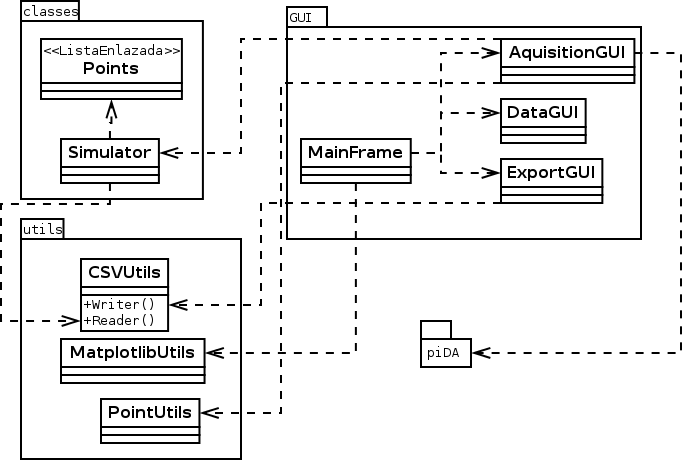
\includegraphics[width=1\textwidth]{classes.png}
\end{slide}

\subsection{Diagrama de refresco de la gráfica.}
\begin{slide}
	\centering
	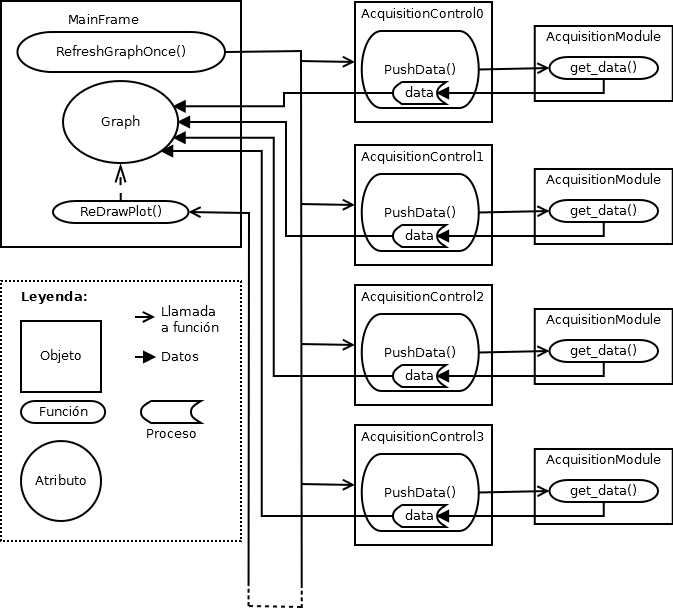
\includegraphics[scale=0.35]{graph-refresh_diagram.png}
\end{slide}

\subsection{Diagrama de redibujado de la gráfica.}
\begin{slide}
	\centering
	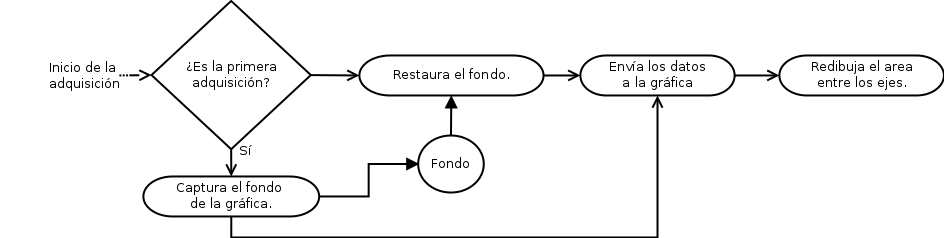
\includegraphics[width=1\textwidth]{graph_redraw-diagram.png}
\end{slide}

\subsection{Acceso a los datos del interfaz: Secciones críticas.}
\begin{slide}
	\centering
	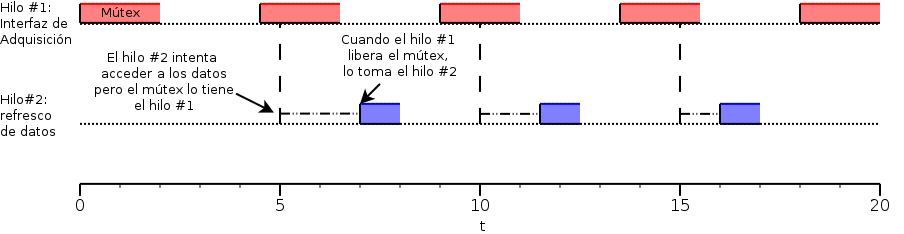
\includegraphics[width=1\textwidth]{diag-sincronia.png}
\end{slide}

\section{Resultado final.}
\subsection{piDA Graphic Interface.}
\begin{slide}
	\begin{center}
		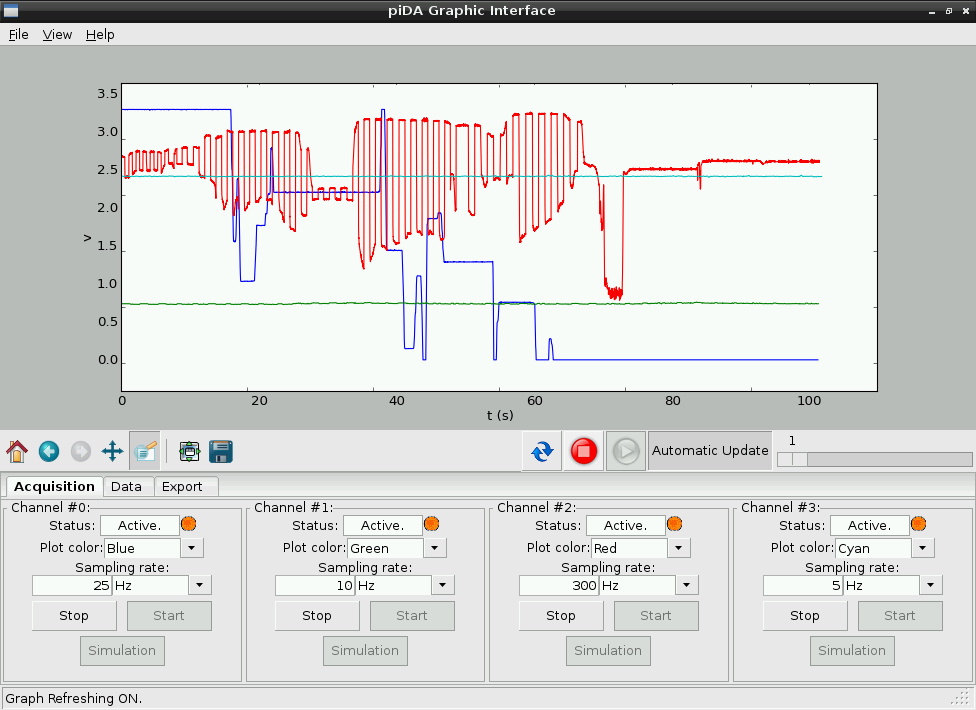
\includegraphics[scale=0.28]{img/pida_4ch_sample.png}
	\end{center}
\end{slide}

\subsection{Evaluación.}
\begin{slide}

\begin{minipage}{.54\textwidth}
\begin{itemize}
	\item Se han evaluado las limitaciones de la solución.
	\item Existe un cuello de botella en el protocolo de E/S.
\end{itemize}
\end{minipage}
\begin{minipage}{.40\textwidth}
  \begin{tabular}{| c | c |}
  	\hline
  	Canales & $ \sum F_{max} $ 	\\ \hline
  	1			&	1135.869				\\
  	2			&	1256.541				\\
  	4			&	1286.831				\\	 \hline
  \end{tabular}
  \end{minipage}
  
  \vspace{2ex}
  En la tabla se representan las frecuencias máximas que se han obtenido en las pruebas.
\end{slide}

\section{Conclusiones y líneas futuras.}
\begin{frame}[environment=slide]
\frametitle{\insertsectionnumber.\insertsection}
	\begin{itemize}
		\item Líneas futuras.
		\begin{itemize}
				\item Adición de nuevas funcionalidades.
				\pause
				\item Optimización de la solución.
				\pause
				\item Implantación en los laboratorios. 
				\pause
				\item Explotación comercial.
				\pause
		\end{itemize}
		\item Conclusiones.
		\begin{itemize}
				\item Se ha demostrado que se puede realizar una solución alternativa al equipo actual con un coste sensiblemente inferior.
				\item El trabajo colaborativo del proyecto paralelo ha sido una experiencia muy positiva.
		\end{itemize}
	\end{itemize}
\end{frame}

\section{Demostración del programa.}

\begin{frame}
\centering
\Huge{¿Preguntas?}
\end{frame}

%\begin{frame}
%\frametitle{Anexo I: Raspberry Pi.}
%Etc.
%\end{frame}
\end{document}

